

\documentclass[10pt, conference, compsocconf]{IEEEtran}
\usepackage{cite}
\usepackage{graphicx,float,wrapfig}
\usepackage{listings}
\usepackage{xcolor}
\graphicspath{ {images/} }
\usepackage{wrapfig}
\usepackage{tabularx}
% Please add the following required packages to your document preamble:
\usepackage{booktabs}
\usepackage[normalem]{ulem}
\useunder{\uline}{\ul}{}
\usepackage{url}
\usepackage{hyperref}
\usepackage[flushmargin]{footmisc}


% correct bad hyphenation here
\hyphenation{op-tical net-works semi-conduc-tor}


\begin{document}
%
% paper title
% can use linebreaks \\ within to get better formatting as desired
\title{Design RESTful Data Service for Data Analytics}


% author names and affiliations
% use a multiple column layout for up to two different
% affiliations
\author{\IEEEauthorblockN{Yun Zhang\IEEEauthorrefmark{1}\IEEEauthorrefmark{2},
		Liming Zhu\IEEEauthorrefmark{1}\IEEEauthorrefmark{2},
		Xiwei Xu\IEEEauthorrefmark{1}\IEEEauthorrefmark{2},
		Shiping Chen\IEEEauthorrefmark{1}\IEEEauthorrefmark{2},
		An Binh Tran\IEEEauthorrefmark{1}}
	\IEEEauthorblockA{\IEEEauthorrefmark{1}Data61, CSIRO, Sydney, Australia \\
		Email:\{Firstname.Lastname\}@data61.csrio.au}
	\IEEEauthorblockA{\IEEEauthorrefmark{2}School of Computer Science and Engineering, University of New South Wales, Sydney, Australia}
	}

\maketitle


\begin{abstract}
Data service APIs provide a uniform and filtered access to data. However, existing \textit{one-size-fits-all} API design for data services is often inefficient for data analytics driven data retrieval because it focuses on the underlying data sources rather than the data analytics needs. The \textit{one-off} API representations lack support for different patterns of data retrieval, and do not leverage hypermedia and data packaging techniques used in RESTful API design. Besides, current data service APIs are designed and configured statically rather than generated dynamically based on data analytics needs in different contexts. Lastly, context information about the origin, scope, and usage of the data provided is seldom considered in data service design.


In this paper, we propose an analytics-focused API design for data services. First, a set of RESTful conversation models are introduced to depict the interactions between data consumers and data sources for different data retrieval patterns. Second, following HATEOAS principle of REST, a navigational model is designed to enable dynamic generation of APIs and navigation among them.  Finally, data package technique is extended to facilitate efficient and flexible data retrieval. We evaluate our approach using a case study and make a comparison analysis between our approach and conventional DaaS (Data as a Service) RESTful APIs. The evaluation shows that our approach is more efficient and effective for data retrieval in data analytics.


\end{abstract}

\begin{IEEEkeywords}
Data analytics; Data service; REST; Data package

\end{IEEEkeywords}

\IEEEpeerreviewmaketitle



\section{Introduction}
% no \IEEEPARstart
A large amount of data has been published on the web for the last decades, which brings great analytic values across both industries and academia. For example, in Twitter, more than 1 million tweets are published every 10 minutes. Another example is government open data platforms, like data.gov.au\cite{dataGov}, which already shares over 20 thousands of datasets for free. How to properly and efficiently retrieve these data for data analytics is becoming a hot issue\cite{jagadish2014big}\cite{sharda2014businesss}.

To analyse a big dataset, data analysts often start by exploring data before knowing exactly what they are looking for. It is not pragmatic to download the whole large dataset before performing any exploratory analysis. Instead, it is desirable to allow analysts to have a glimpse into the data through a sequence of exploratory queries before the retrieval for further analysis\cite{khan2014divide}. Data exploration,
which is a interactive process to retrieve data, allows the analysts issue a query, receive a response, and then iteratively interact with the data system to refine their query based on the response from the system and domain knowledge\cite{idreos2015overview}. The other two commonly used data retrieval patterns are batch and stream retrieval. In batch retrieval, data is collected to do some relatively time consuming data analytics tasks. In stream retrieval, a query is being repeatedly executed over a stream of data at real-time. Thus, rather than batch processing, stream retrieval pattern allows users to analyze the data-in-motion. 
%Stream analysis allows user to analyze the data in-motion.

Since data exploration is labor-intensive and repetitive, it would be beneficial for analysts if the value-added data derived from the exploration stage could be shared and reused in future. The data analysts can share the results from the earlier exploration to better streamline the data analytics pipeline. To enable more efficient data sharing and reuse, it is very important to provide provenance information of data source so that data consumers are informed about what sort of earlier manipulations have been done to the data.

%Since data exploration is labor-intensive and repetitive, it is beneficial for the analysts if this value-added data derived from the exploration stage could be shared. If shared data also contains information about where it is derived from, the data analysts can better streamline the data analytics pipeline. Thus, it is very important to provide the provenance information of a data source so that data consumers are informed about what sort of earlier manipulations have been done to the data.



%First, the existing data services provide \textit{one-size-fit-all} solution -- they answer questions about the data according to the underlying database schema and pre-assembled index. They are not driven by the requirements of data retrieval for data analytics\cite{dillon2013towards}. Second, these data services are isolated and static -- they only support \textit{one-off} queries. These sevices do not leverage HATEOAS (Hypermedia as the Engine of Application State) or provide data analytics specific semantics to enable service self-discovery. Third, these sercvices do not have a standard mechanism for providing context information about the data such as origin, scope, and usage. Data analysts cannot be informed about what data exist, how the data are derived and used. As a result they cannot infer whether these processed data can be reused. 

Data services provide unified, scalable and filtered interfaces for data analysts to retrieve data\cite{borkar2006xml}. Many companies and platforms, like Twitter, Google, and CKAN\cite{CKAN} offer data service APIs that provide simple and easy-to-use access to some of their resources. Data services allow third-parties to easlily integrate the data resource into their applications. However, these conventional interfaces fall short on supporting responsive, interactive, and comprehensive data retrieval for analytics. First, the existing \textit{one-size-fit-all} data services are designed to answer questions according to the underlying database schema and pre-assembled index, rather than being driven by the requirement of data retrieval for data analytics\cite{dillon2013towards}. Second, the \textit{one-off} data queries are isolated and static, which does not leverage the HATEOAS (Hypermedia as the Engine of Application State) principles of REST. It does not support service self-discovery. Third, there is no standard mechanism to provide context information about the origin, scope, and usage of the data behind data services. Data analysts cannot be informed about what data exists, how the data is derived and used, and as a result they cannot infer whether these processed data can be reused. 

%To effectively and efficiently assist users to retrieve data in data analytics, 
In this paper, we propose a data service API design driven by analytics's need. Our contributions include (1) a set of RESTful conversation models for the interaction between data consumers and resources, (2) a navigational data model to help discover and  generate data service API dynamically, and (3) a mechanism using extended data package to contain, publish and share data processing scripts and data context information. We evaluated the proposed API design through a feasible case study and discussion about quality attributes. The evaluation shows that our approach....

The rest of this paper is organized as follows. Section~\ref{background} describes some related work. Section III introduces the data service design including the three conversation models, the navigational model and the extension of data package. Section IV uses a case study to evaluate our API design. Section V concludes the paper.

% You must have at least 2 lines in the paragraph with the drop letter
% (should never be an issue)
\section{Background and Related Work}
\label{background}
REST (REpresentational State Transfer) \cite{fielding2000architectural} is an architecture style for designing web applications. Following REST design principles, data service is identified by URI as a resource, and interacted with client applications by request-response messages. Protocols and Structures for Inference (PSI)\cite{PSI} specifies a RESTful architecture for presenting machine learning and related moudules as RESTful web services, whereby the data access is wrapped as data service named relation. However, the relation does not indicate how to discover a related data service for data exploration.

Database-as-a-Service (DaaS) has emerged as a new paradigm in the cloud computing environment. Many commercialized databases, like Amazon SimpleDB\cite{Amazon} and Microsoft SQL Azure\cite{Azure}, provide accessible data service APIs to their data stores.  ODBAPI\cite{sellami2014odbapi} is a uniform REST API to execute CRUD (create, read, update, delete) operations across various relational and NoSQL data stores. HTSQL\cite{HTSQL} enables accessing SQLServer via HTTP arbitrarily, which is an advanced query language on the web designed for data analysts who have complex inquiries across relational databases. However, these CRUD-based data services are designed and implemented according to database schemas and pre-assembled indexes without reference to the underlying domain application protocol.

In order to build a domain application protocol over HTTP which is domain agnostic in the web application, some additional, explicit semantics are needed\cite{wilde2011rest}. In the Semantic Web, semantics are described by ontologies written in RDFS and OWL, while RESTful implementations encode semantics by annotating hypermedia with link relations\cite{page2011rest}. 

Hypermedia as the Engine of Application State (HATEOAS) which is the hypermedia constraint, requires that the service should embed links in its responses. The links represent the next possible actions that the client can take\cite{fielding2000architectural}. However, there is a “semantic gap” for clients to be navigated by hyperlink automatically. In order to remedy this design flaws in HATEOAS implementation, some hypermedia specifications such as AtomPub\cite{AtomPub} and OpenSearch\cite{OpenSearch} are tailored to achieve the specific application goals. However, the semantics of these domain-specific media types are implicit and generic\cite{Robinson2011}. AtomPub is designed to cover all the collection-based APIs but cannot reflect different application semantics. Microsoft’s Open Data Protocol (OData)\cite{OData} derived from AtomPub defines the protocol semantics for filtering and sorting a collection of data, using a query language similar to SQL. 

However, the semantics of the relationship between resources focus on data instead of analytics operations, and the related metadata services only present limited description documents\cite{richardson2013restful}. Our approach fills this semantic gap by specifying the domain application protocol of data exploration in analytics and bringing this protocol into the HATEOAS implementation of our services. 

Metadata provides self describing information about web resources in REST architecture, which enable automatic processing of web resources\cite{Hernández2011}. However, the metadata is sent in headers of HTTP message and restricted to provide information about the syntax used in the resource representation. In addition, the semantics about the origin, scope, and usage of the data is less considered. Ground\cite{hellerstein2017ground} is a data context service that supports collecting, publishing and querying the metadata information from applications, behavior, and change of data context, but it is implemented as a system without consideration of RESTful API presentation. Data package is a collection of datasets, metadata information and other data files. Data package protocol\cite{dataPackage} defines an open standard for the format of package, which guide users to share and manage distributed dataset using data package. However, there is no guidance on how to apply data package for exchanging metadata in RESTful services.
\section{Data Service Scenario}
\begin{figure}[th]
	\centering
	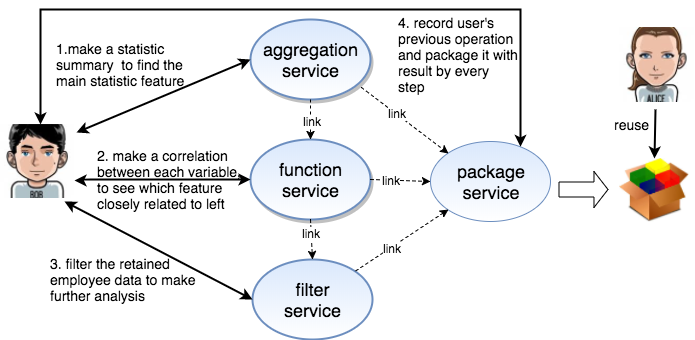
\includegraphics[width=0.45\textwidth]{scenario.png}
	\caption{Data Exploration Scenario Using Data Service}
	\label{fig.1}
\end{figure}
We use a practical human resource analytics scenario to show how data services aid in data exploration and facilitate collaboration. The purpose of the analysis is to help a company understand why some of their best and most experienced employees are leaving prematurely and predict who will leave in future. 

Analyst Bob first makes a request of statistic summary of the data provided by the company, investigating the sum, average, min, max and medium of numeric attributes respectively. Apart from the result of aggregation, the data service also returns the URIs of services for all the possible next steps. Bob then selects the function service to make the second request to discover a correlation between each pair of attributes. The results show that on average, employees who left the company have lower satisfaction levels. After knowing all the features of employees who have left, Bob uses the filter service to retrieve the data about valuable but left employees with an evaluation result above average performance, or spend at least four years in the company, or were working on more than five projects at the same time and still have left the company. After developing insight from the data, Bob uses these data to conduct an analysis model to predict who will leave.
\begin{figure*}
	\centering
	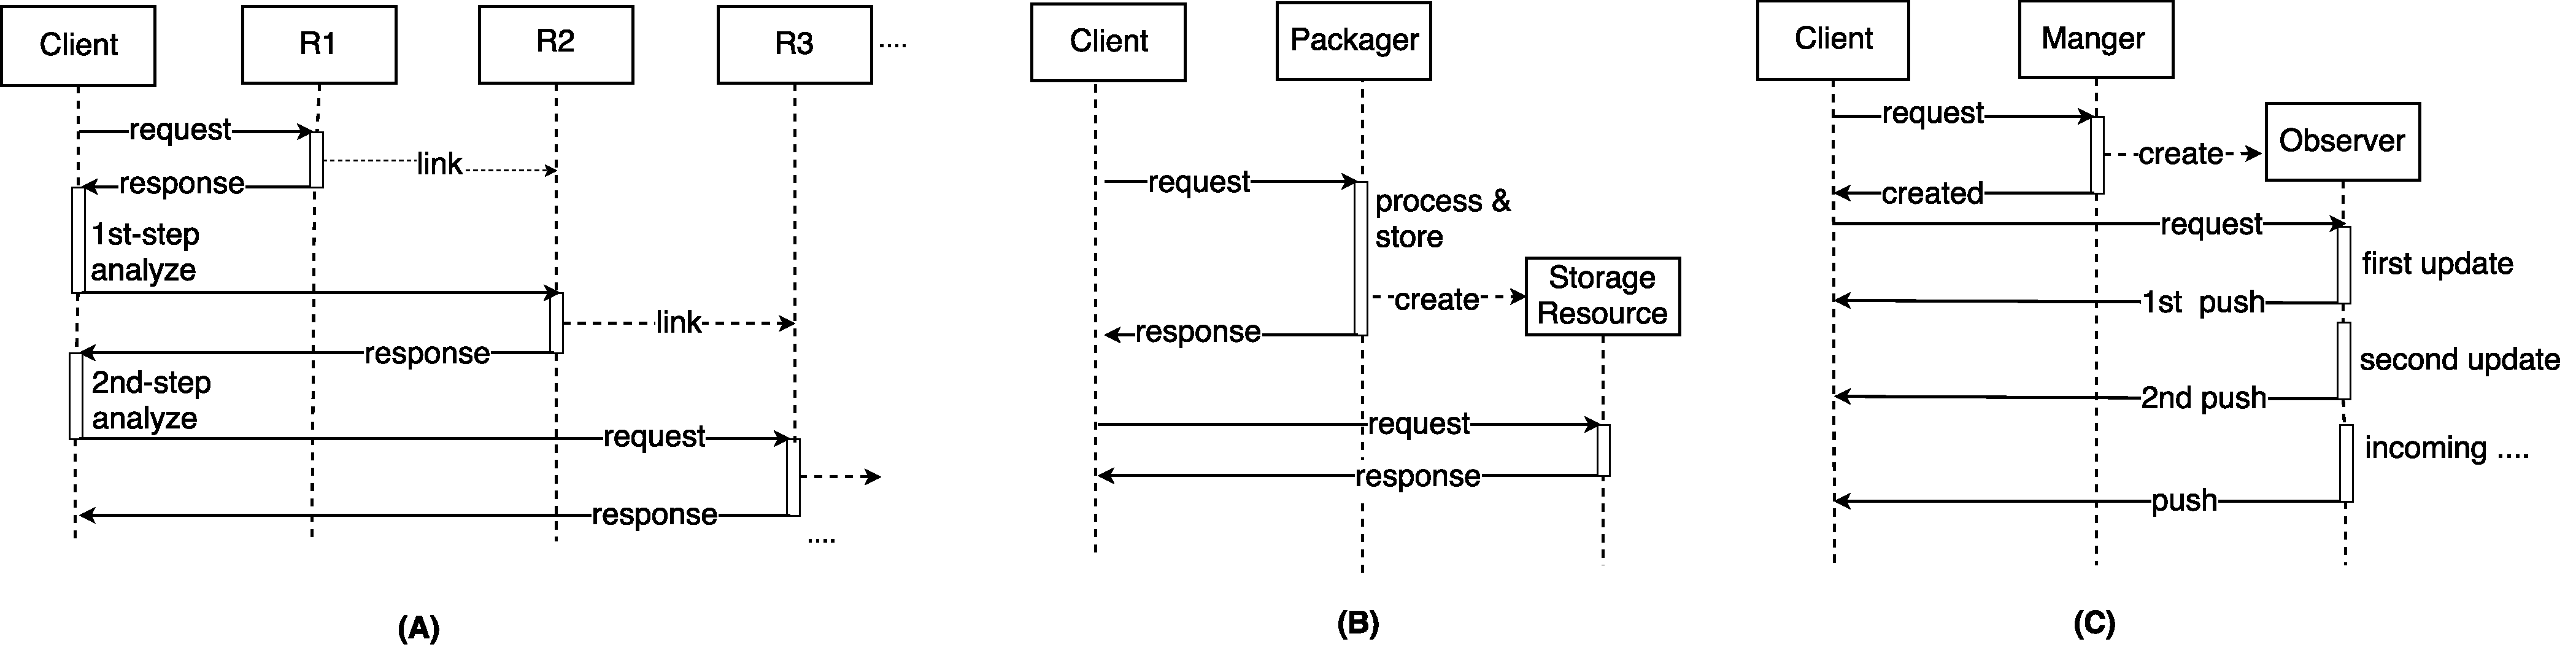
\includegraphics[width=1.0\textwidth]{ThreeConversationModels}
	\caption{Conversation Models}
	\label{fig.2}
\end{figure*}
After Bob finishes explorative analysis, he invoke package service to wrap his data exploration process as a data package and share it on the web. The data package is then discovered by Alice to do further analytics without preparing data from scratch. Alice can also reprocess the operations included in the package to verify Bob’s exploration result. Even, she can leverage Bob's explorative analysis operation referred service to extend and constrct her own operation. This style of work could be repeated, by producing and sharing Alice's data package for another analyst.

There are three main benefits from using the data service to realize data exploration. First, from the data consumers’ (like Bob and Alice) perspective, pushing computation to the data is more efficient than pulling the whole data out for computation. Therefore, it is desirable to move the basic and frequently used analytic operations to the data sources and wrap them as services. The resources interconnected via hyperlinks could navigate analysts to find the data they need quickly and preciously. Second, from the data publishers’ (like the company) perspective, they can expose lightweight data features for analytics to protect data privacy and commercial interests rather than open the whole data. Lastly, the data package enables data consumers to share the result of their exploration as data publishers, and thus brings the benefit of reusability, flexibility and customizability.
\section{Service Design}
\subsection{Conversation Models}

RESTful conversation\cite{haupt2015conversation} is a sequence of interactions between a client and resources. The conversation route is controlled by the resources following the HATEOAS principle and driven by the client. Three RESTful conversation models of the data retrieval patterns for data analytics are depicted by UML sequence diagrams.

\subsubsection{Interactive Conversation Model}
In order to reduce the computation cost and improve the timeline of analysis, the interactive analytics involves the human insight into the process of data analysis. As shown in Fig.2(A), a \textit{client} issues the first query to the resource R1, the response of R1 contains the requested data and the possible links that the \textit{client} could select. The \textit{client} analyzes the returned result, and then chooses the link pointing to the resource R2. Again, this conversation repeats until the result is satisfied.


\subsubsection{Batch Conversation Model}
Batch retrieval means a group of operations are executed for retreiving data in batch. As the task might be time-consuming, the request can be processed asynchronously while a link pointing to the dataset is returned immediately to the client. The main interactions of batch conversation model are shown in Fig.2(B), a \textit{client} makes a request to the resource \textit{packager} which is responsible for extracting data from the data source. \textit{Packager} generates the data package and stores it into the remote storage, meanwhile responding instantly with a hyperlink referring to the to-be storage resource. The \textit{client} keeps polling the data status from the \textit{storage resource}, until the data is ready.

\subsubsection{Streaming Conversation Model}
In the streaming data retrieval, a client can receive the real-time updates or events occurred from the resource. This pattern allows analysts to analyze the data-in-motion. The streaming conversation model involves three roles: the client, the manager and the observer. Specifically, as shown in Fig.2(C), the \textit{client} makes a request on the resource \textit{manager} with parameters like window, interval or operations in the representation. The \textit{manager} identifies the \textit{client}’s interest, creates the \textit{observer} based on requirement of the \textit{client}, and then responds the link of the \textit{observer}. Afterwards, the \textit{observer} monitors the state of the data and delivers the user-defined stream data and push-like notification in real time.
\subsection{Service Architecture}
\begin{figure}[th]
	\centering
	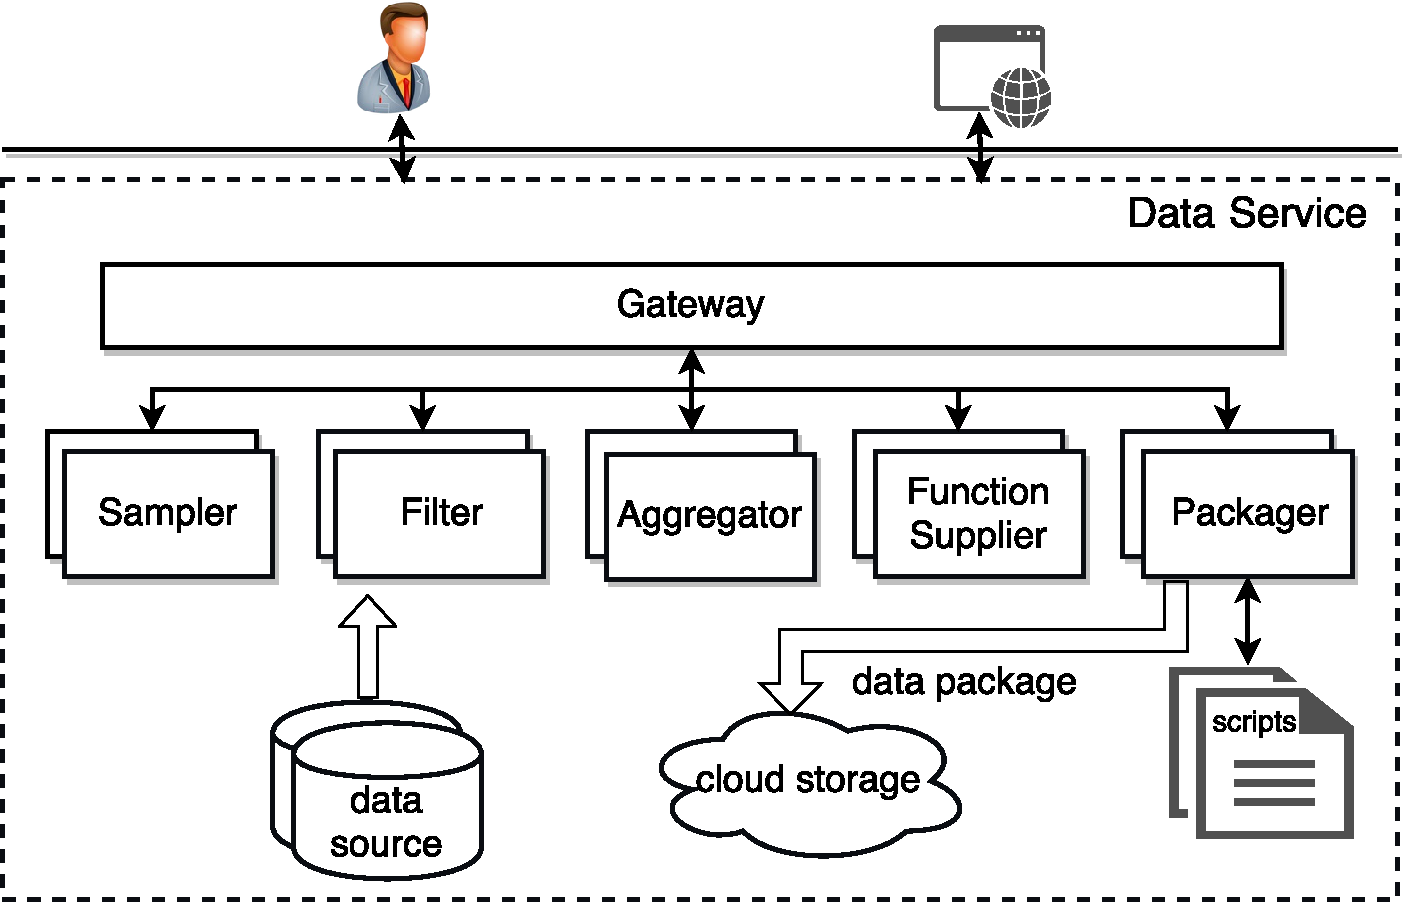
\includegraphics[width=0.5\textwidth]{serviceArchitecture.pdf}
	\caption{Data Service architecture}
	\label{fig.3}
\end{figure}
In this section, we introduce the service architecture with the main resources. As shown in Fig.3, the main components in our architecture are the \textit{gateway, filter, aggregator, sampler, function supplier} and \textit{packager}. We propose a navigational model to describe the relationship of the main resources in the domain of data analytics and motivate the idea to use this model as a modeling tool for REST APIs. We apply data package technique into our data services and showcase its usage and advantages in a data analytics pipeline environment. 

    \subsubsection{Key Resources}

\textbf{Gateway} is a self-describing resource that exposes the metadata defining data schema and other information like data type (for example, dynamic, static), data size, attributes and description about this dataset, which helps the data analyst have an initial understanding about the dataset. Further, the \textit{gateway} acts as a role of discovering related resources about the dataset. 

\textbf{Filter} filters the data based on dimensions and measures which are presented based on non-numeric attributes and quantitative attributes. Dimensions represent which attributes of data that can be extracted while measures represent the query schema that is used to extract the subset or transformation of the dataset. Dimensions are divided into atomic and composite dimensions according to the data features. The composite dimension is hierarchical, for example, a time dimension is composed of year which consists of four quarters containing all months. On the other hand, the measures are not only based on the built-in query schema but also can be a combination of measures expressed in mathematic operation as well as statistics functions.

\textbf{Aggregator} allows users to have a whole characteristic of the large subset of the data without extracting specific data items. It can perform aggregation function over one attribute’s values and group by the attribute’s name. The aggregation queries have constraints based on the attribute’s numeric or non-numeric features.  

\textbf{Sampler} provides diverse sampling methods, like random sampling, to sample a specified size of data with or without placement, which allow analysts to quickly build and test their models within a sample of data that can fit into the client’s memory. The sample size and specific sample methods are defined by users. 

\textbf{Function Supplier} provides a set of functions, which effectively assist data analysts as auxiliary means. For example, \textit{correlation} is for understanding the relationship between attributes; \textit{isnull} is a necessary function for data cleansing, which is used to check for the missing value to help analysts know the data quality. Then analysts can take three methods for missing values in our data services: drop the record with missing values, drop variables and fill in the missing value with a default or user-defined value. All these methods can be supplied by the \textit{filter} while retrieving data.

\textbf{Packager} retrieves the big volume data, wraps them with optional primitive operations which are presented as scripts into package, and then store them in external storage. Using the packager, the data consumer can acquire a targeted subset of dataset in batch along with the optional scripts provided by the data publisher. These scripts can be used to pre-process the data and accelerate the forthcoming analysis work. We discuss more detail as below.
\subsubsection{Navigational Model}
The resources in the service architecture are interconnected to each other according to the context. A navigational model which defines the domain application protocol of data exploration in analytics is designed to assist clients to form their queries for interactive exploration of large datasets. Based on the navigational model, data service can recommend possible next steps for the query session, and provide the information of relationship between the resources in the context of data analytics. 

The navigational model is shown in Fig.4. The circles represent the resources introduced in last section, while arrows correspond to the relationships between the resource API templates. The relationships across resources are categorized into four types: \textit{narrow down}, \textit{summary}, \textit{relate} and \textit{wrap up}. Specifically, \textit{narrow down} means zoom into the data from less detail to more detail. Users could be guided to the \textit{filter} API template by the \textit{narrow down} link to query detailed data from summarized data based on the data distribution or extreme value provided by the \textit{aggregator} or the \textit{sampler}. Conversely, users can zoom out the data that are of little interest to discover other attributes through \textit{sampler} or \textit{aggregator} API template guided by the \textit{summary} link. The \textit{relate} link presents auxiliary services, for example, some statistic functions like correlation, standardization and distribution. During the process of data exploration, \textit{wrap up} appears in every stage to refer users to the \textit{packager} API template when the returned data are too large for the client memory or the users wants to download the whole data with previously recorded data exploration track.
\begin{figure}
	\centering
	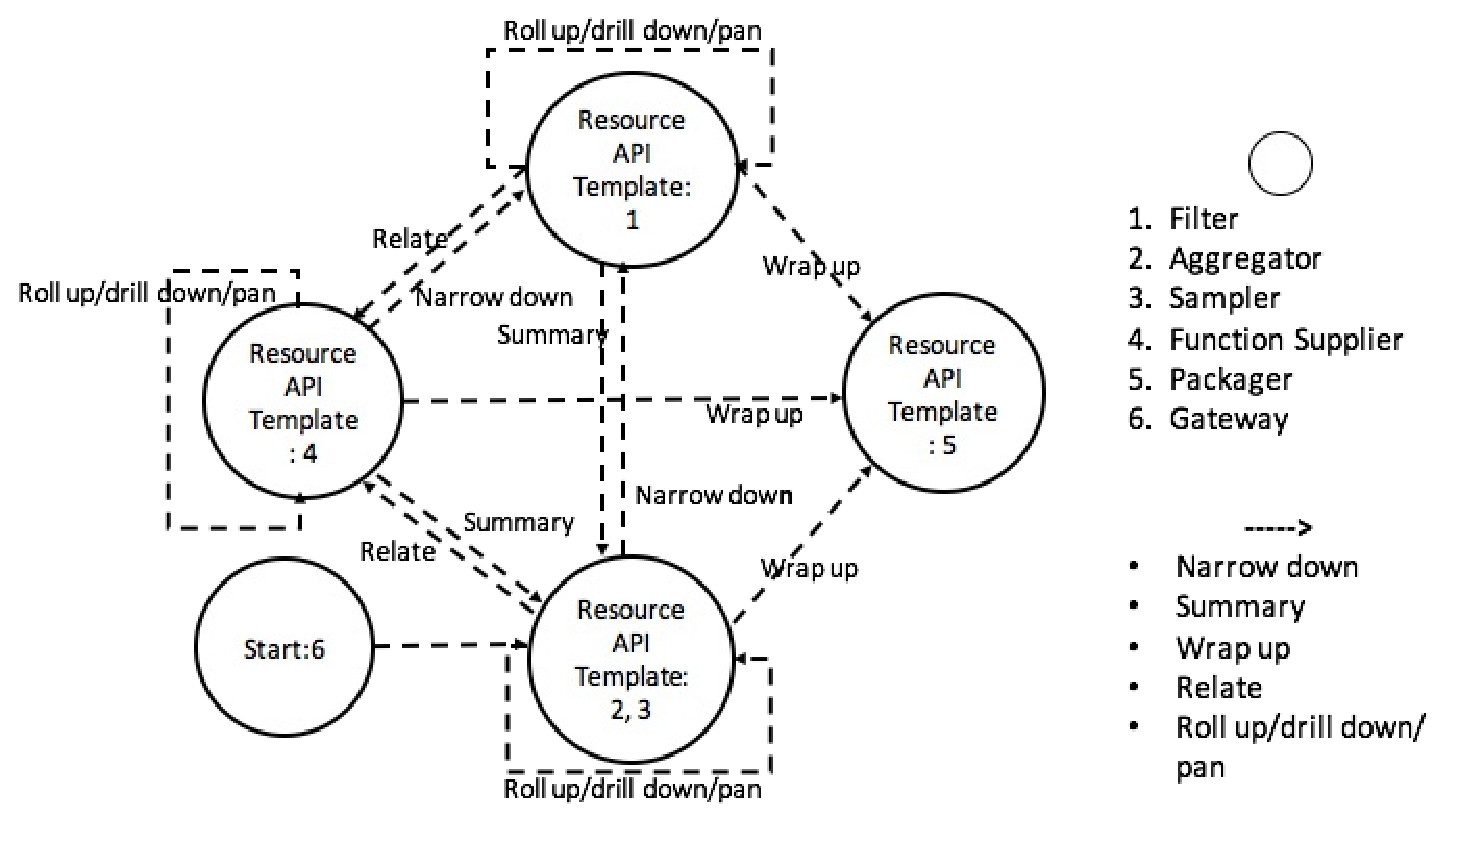
\includegraphics[width=0.5\textwidth]{navigationalModel.pdf}
	\caption{Navigational Model}
	\label{fig.4}
\end{figure}
When focusing on one resource, the user can send a sequence of requests to the resource API template adjusting the parameter values until she is satisfied with the results. Alternatively, such a query session could be accelerated by our navigational model through parameter prediction  \textemdash  parameter values can be used to instantiate the API templates through analyzing the past parameters provided by user. We generalize three types of relationship based on users navigational activates including \textit{Roll up, drill down }and \textit{pan}. Concretely, \textit{drill down} provides a more detailed view by either stepping down a hierarchy within a dimension or introducing additional dimensions or attributes through changing the parameters. For example, when viewing the salary data of Australia, a drill down link provides the service querying the data of different states like NSW (New South Wales), QLD (Queensland), etc. A further \textit{drill down} on NSW may display data of Sydney. It also can restrict the results in \textit{aggregator} by tweaking the “where” and “having” conditions. \textit{Roll up} is the reverse of \textit{drill down}: it means climbing up a concept hierarchy for a dimension, reducing the dimensions or relieving the conditions in measure. \textit{Pan} allows users to change the angle they observed by changing the dimensions of data or the operations used.

The navigational model incorporates the analytics domain semantics into HATEOAS. Specifically, the \texttt{links} property is used to represent all the related actions and resources for each resource with which clients can interact. \texttt{links} is defined as an array of Linked Description Objects(LDOs) in JSON Hyper-Schema\cite{JSONSchema}, which obeys HATEOAS constraint and assist discover all the related resource API templates with the current resource API.  Each LDO at least contains one \texttt{href} property, which is the target of the link, and a \texttt{rel} property indicating the relationship between the linked resource and the current resource. Users could effectively make a data exploration by looking if the representation has embedded \texttt{links} to the next resource. 

The navigational model involves in both dynamical discovery and generation, which enable discover the resource API template driven by client while generate the API parameters based on the previous input from client. We present their schemas of Links separately in listing 1 and listing 2. 

As shown in listing 1, each \texttt{links} comprises of \texttt{rel} which present the meaning of related action, and \texttt{href} which points to the location of resource. The \texttt{rel} indicates “\textit{relate, summary, narrow down} and \textit{wrap up}” for resource APIs' dynamic discovery. The \texttt{method} and \texttt{schema} properties specify the HTTP method and data format for the input. Afterwards, client can send a HTTP OPTIONS request to acquire further assistance on how to form a specific API. Listing 2 defines the schema of \texttt{links} for generating the specific resource APIs. According to the different semantics of \texttt{rel}, the new parameters are intelligently generated based on the measures and dimensions in the \texttt{base}, and form a new resource API as a \texttt{href} property for client. The \texttt{rel} indicates \textit{roll up, drill down} and \textit{pan} for resource APIs dynamic generation.
\lstdefinestyle{mystyle}{
	breakatwhitespace=false,         
	breaklines=true,                 
	captionpos=b,                    
	keepspaces=true,                 
	showspaces=false,                
	showstringspaces=false,
	showtabs=false, 
	basicstyle=\fontsize{7}{8.5}\ttfamily
}
\lstset{style=mystyle}

\begin{lstlisting}[language=python, caption=HyperSchema of Links for Dynamical Discovery]
{
	"$schema": "http://json-schema.org/draft-04/schema#",
	"title": "Schema defining links between resources",
	"type": "array",
	"items": {
	"links": [{
		"rel": "narrow down",
		"href": "/filter",
		"method": "GET"
	},{
		"rel": "summary",
		"href": "/aggregator",
		"method": "GET"
	},{
		"rel": "relate",
		"href": "/functionSupplier",
		"method": "GET"
	},{
		"rel": "wrap up",
		"href": "/packager",
		"method": "POST",
		"schema": {}
	}]
	}
}
\end{lstlisting}
\begin{lstlisting}[language=Python, caption=HyperSchema of Links for Dynamical Generation]
{
	"$schema": "http://json-schema.org/draft-04/schema#",
	"title": "Schema defining links within one resource",
	"base": "/{resource}?{measures,dimensions}",
	"type": "array",
	"links": [{
		"rel": "drill down",
		"href": "/{resource}?{measures,added_dimensions}",
		"method": "GET"
	},{
		"rel": "roll up",
		"href": "/{resource}",
		"method": "GET"
	},{
		"rel": "pan",
		"href": "/{resource}?{new_measures,new_dimensions}",
		"method": "GET"
	}]
}...
\end{lstlisting}

\subsubsection{Data Package}
We adopt data package as a media type to allow users to customize and reuse the data exploration process to support more flexible and efficient data retrieval. By using the packager resource, data providers can package the processed data with related scripts. For example, assume that the World Bank publishes a dataset about middle income countries together with a script that calculates the middle income based on annual analysis. Thus, the data analyst can effectively query data and perform analysis based on the scripts included in the data package. 

Fig.5 gives an overview of the extended data package, which may contain (1) data such as tables and files stored remotely in cloud storage or in the package. Data is classified into source data, result data, query data according to their purposes, (2) scripts processing and analyzing data, which are written by the data provider or generalized by the data service in any cross-platform languages like Python or Java, and (3) metadata describing the structure and the contents of the package, as well as the relationship between the data and scripts and the data context information. Specifically, a basic metadata consists of the following properties: 
\begin{figure}[th]
	\centering
	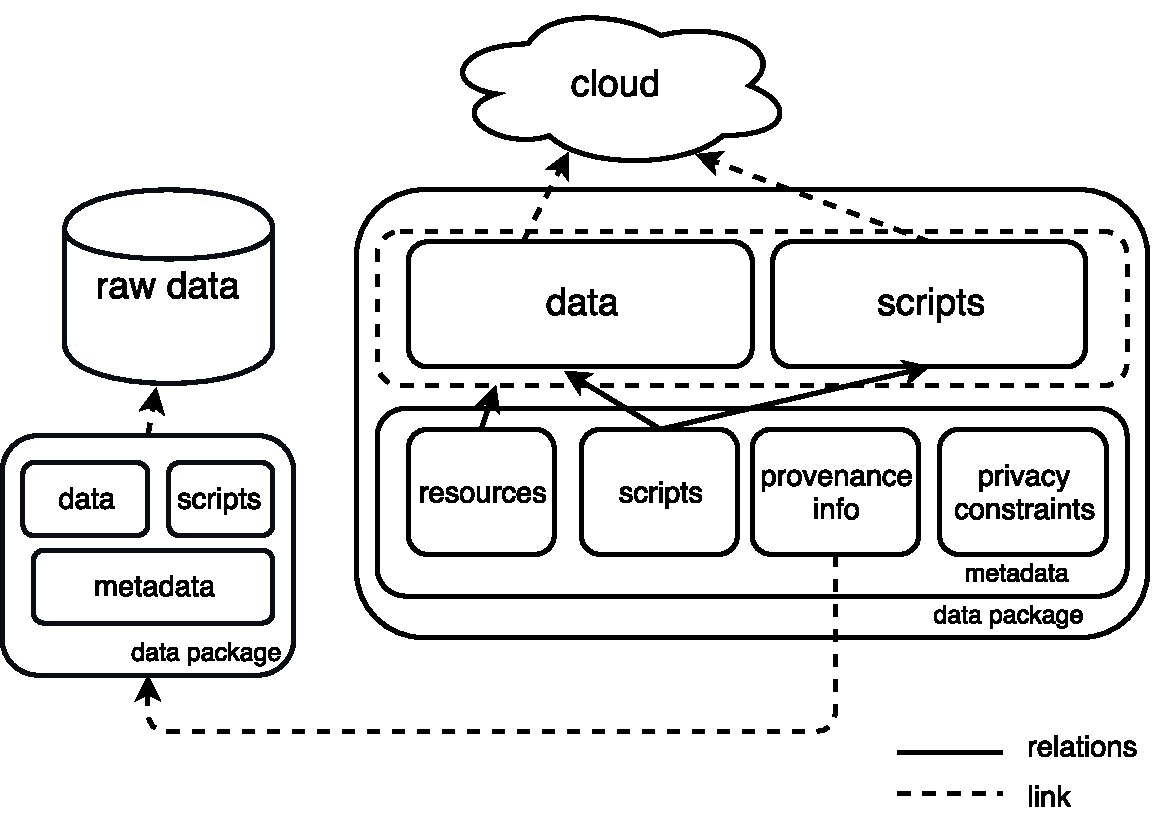
\includegraphics[width=0.45\textwidth]{dataPackageStructure.pdf}
	\caption{Data Package Structure}
	\label{fig.5}
\end{figure}
\begin{itemize}
	\item \textit{Resources} describe and locate all packaged data. The descriptor could be in JSON or XML format while the paths could be a local path within package(inline) or URLs pointing to remote storage(non-inline). 
	\item \textit{Scripts} indicate the location of inline and non-inline scripts and specify the purpose of the scripts on the data sources and the correlation among scripts and data. This property helps analyst understand what operations have been done on which datasets.
	\item \textit{Provenance information} is a sequence of links pointing to the previous data packages from which current package is generated. It records the package chain linked by the hypermedia to allow users to trace the data usage in the data pipeline. 
	\item \textit{Privacy constraints} record the privacy constraints imposed on the data of current package. When data providers apply privacy-enhancing techniques to generate anonymous data or expose their data partially, their operations could be informed to analysts so that they can take corresponding tactics in their analysis.
	\item \textit{Other descriptor} includes data schema, author, contributor, version, etc. 
\end{itemize}	

A simplified data package example in JSON is shown in Listing 3. The required properties are listed, others are omitted due to length limitation.
\begin{lstlisting}[language=python, caption=A Data Package Example]
{
	"name": "dataPackage",
	"id": "",
	"sources": [{
		"title":"hr-analytics dataset",
		"path": "https://www.example .com/datasets/hr-analytics"
	}],
	"resources": [{
		"path": "http:/www.example.com/hr-analytics.csv",
		"schema": "{...}"
	}],
	"scripts": [{
		"name": "retreive_good_employee_who_left",
		"path": "",
		"type": "python",
		"resources": ["good_employees_left", ".."]
	}],
"provenanceLogs": [{
		"lastPackage": "",
		"created_in": "06/06/2017",
		"path": "http://example/HrAnalytics/dataPackage"
	}],
"privacyLogs": [{
		"script_name": "",
		"description": ""
	}]
}
\end{lstlisting}

In our data service architecture, the data package takes two roles as below:

\textit{Data package as a resource} As introduced in batch conversation model and the key resources section, the packager can package a big volume set of data into a non-inline resource by a path pointing to the remoted storage. Apart from the link to the data, the scripts inside the package that record the user’s exploration process. Data package can be created through POST and be retrieved through GET. The included data, scripts, and metadata respond to GET, PUT and DELETE respectively.

\textit{Data package as a context service} Data package provides provenance information, the upstream lineage, and the data constraints like privacy compliance policy. For example, data publisher can use a random value perturbation techniques to hide sensitive data by randomly modifying the data values using additive noise while preserving the underlying probabilistic properties of the dataset so that a predictive analysis can be performed. The metadata in the data package describes this manipulation and privacy constraints so that data consumers are more informed on the assumptions of data for later analysis.
\section{Evaluation}
We implement a case study to conduct a comparative evaluation of the proposed data service design for analytics against the traditional DaaS REST APIs with respect to REST maturity, interoperability and self-discoverability. 
\begin{figure*}[h]
	\centering
	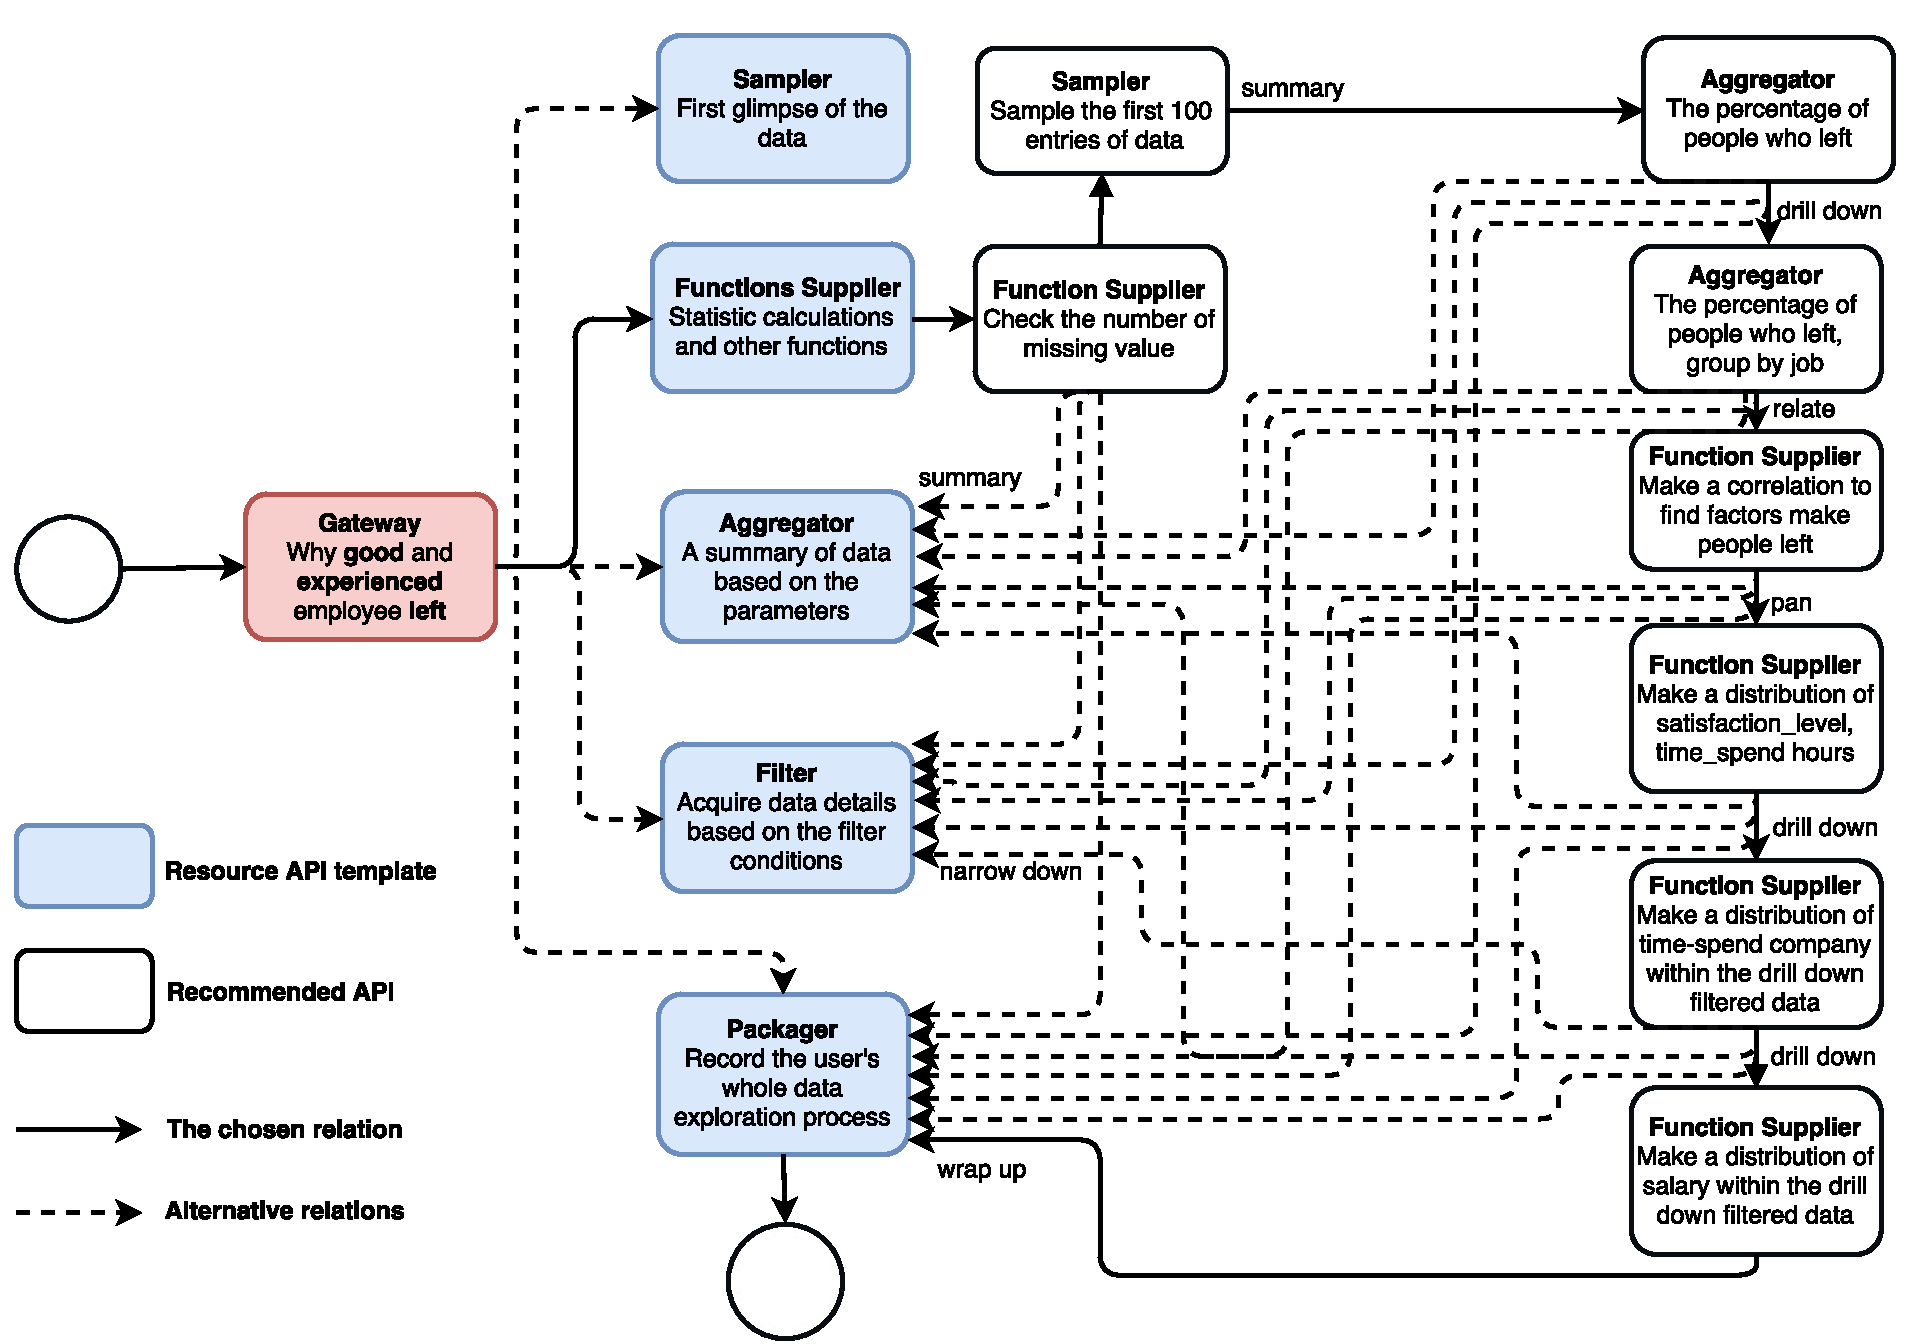
\includegraphics[width=1.0\textwidth]{CaseStudy}
	\caption{HR Analytics Data Exploration Roadmap}
	\label{fig.6}
\end{figure*}
\subsection{Case Study}
We selected one open dataset and its related data exploration process from Kaggle\cite{kaggle} to implement the HR analytics scenario discussed in Section III. 
The RESTful web services are implemented using Apache CXF JAX-RS in java. Figure.6 shows the roadmap of the data retrieval process with the alternative relations and the resources. During the interactive data exploration, each service is automatically discovered and related parameters are intelligently generated. The process can be navigated to the packager for executing multiple operations in batch. 

\subsubsection{Interactive Process}
The analyst starts from \textit{gateway} which responds with a list of resources to be selected. He starts his work from checking the data quality by the resource \textit{function supplier}, which returns the numbers of missing values for the selected attributes,  as well as links indicating the \textit{filter}, the \textit{aggregator}, the \textit{sampler} and the \textit{packager}. Then the analyst sends a GET request to the \textit{sampler} to retrieve a sample data, the returned response contains a defined size of data sample and the URIs of services for all the possible next steps. Next, the analyst chooses the \textit{aggregator} to retrieve the summary information of the data. In each response, apart from a link pointing to the main resource API template, a specific API with predicted parameters will be recommended with an indicative \texttt{href} property. As shown in the Fig.6, when the analyst makes a request of percentage of left people, the response includes a \textit{drill down} link pointing to a predicted \textit{aggregator} API to group left people by their job. Afterwards, he selects the \textit{function supplier} to discover a correlation between each pair of attributes. The results show that on average, employees who left the company have lower satisfaction levels. The returned result guides the analyst to query the distribution of each feature correlated with the left employees. After knowing all the features of employees, the analyst moves to the \textit{filter} to retrieve the data about valuable but left employees with an evaluation result above average performance, or spend at least four years in the company, or were working on more than five projects at the same time and still have left the company. Fig.7 demonstrate the detailed RESTful interactions of data exploration we described above.
\begin{figure*}[h]
	\centering
	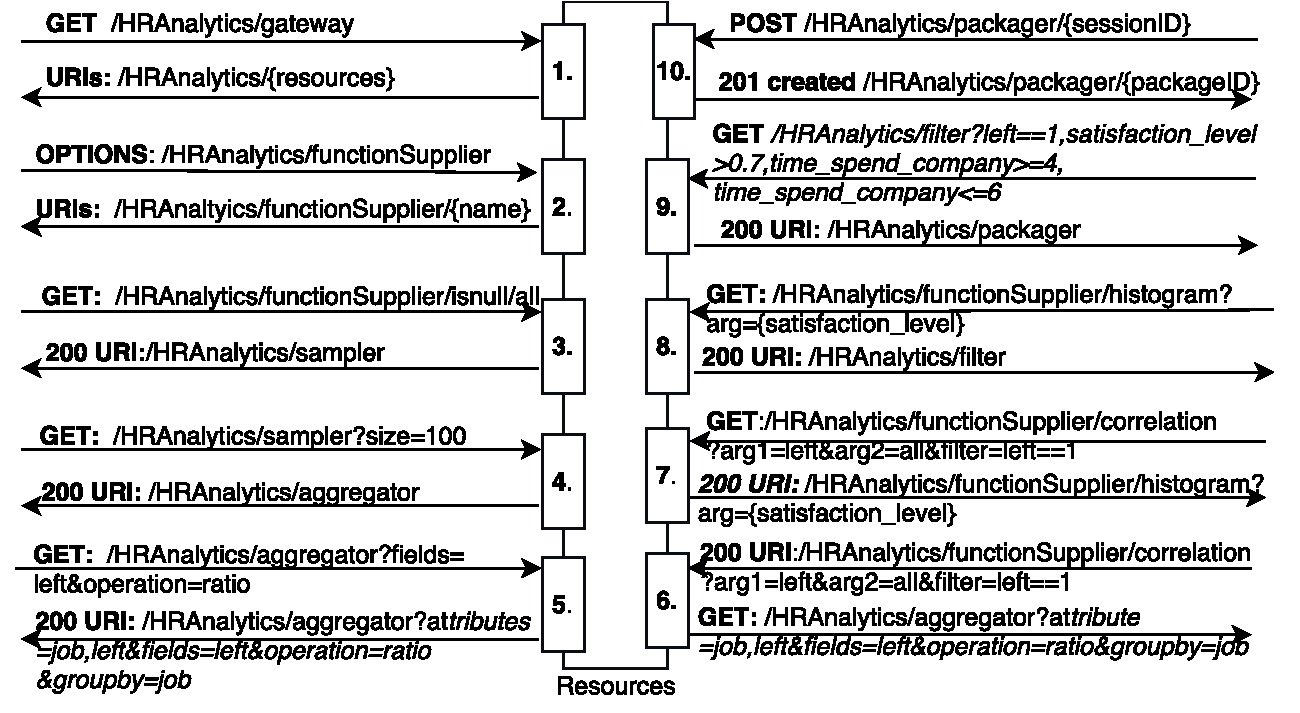
\includegraphics[width=0.8\textwidth]{CaseStudyInteractive}
	\caption{Interactions in the Implementation of the Case Study}
	\label{fig.7}
\end{figure*}
\subsubsection{Batch Process}
After the analyst finishes his exploring the data, as shown in Fig.6, his data exploration process can be wrapped as a script into data package. He can share the data package in any data sharing platform for the purpose of reusability of data exploration.

The data package is then discovered by another analyst to do further analysis without preparing data from scratch. Based on the context information in the package, the second analyst can reprocess the scripts to acquire the initial analyst's exploration result. The content of the POST request is shown in listing 4. The packager will execute the operations in batch in the backend, and return the URI of to-be prepared result. Afterwards, the second analyst will GET the result until the result is ready. 
\begin{lstlisting}[language=python, caption=Asynchronous Interaction with Packager]
POST /HRAnalytics.com/packager
Content-Type: application/json
{
	"script":[{
	"id": "http://localhost:8080/HRAnalytics/functionSupplier/isnull/all", "operation":"GET"
},{
	"id": "http://localhost:8080/HRAnalytics/sampler?size=100",
	 "operation":"GET"},{...}
  ]}
  
response: 201 created /HRAnalytics/packager/{id}

GET http://localhost:8080/HRAnalytics/HRAnalytics/packager/{id}

//result is not ready
response: 202 Accepted Content-Type: application/json
{
	"completed": false
}

//result is ready
response: 200 0k Content-Type: application/json
{
	"completed": true,
	"results": [
{
	"id": "http://localhost:8080/HRAnalytics/functionSupplier/isnull/all",
	"output": "http://localhost:8080/hranalytics/packager/{id}/output_1.json"
	},{
	"id": "http://localhost:8080/hranalytics/sampler?size=100",
	"output": "http://localhost:8080/hranalytics/packager/{id}/output_2.json"
	},{...}  
]}
\end{lstlisting}
\subsection{Evaluation}
\newcommand{\tabitem}{~~\llap{\textbullet}~~}
\begin{table}[ht!]
	\caption{Comparison of information sharing at Semantic level}
	\label{table.1}
	\scriptsize
	\centering
	\begin{tabular}{lll}
		\toprule
		&\quad\quad\quad \textbf{DaaS} & \quad\quad\textbf{RESTful Data Service}  \\ 		
		\midrule
		\textbf{Analytics} & Mapping to the & Conform to data retrieval patterns \\ 
		\textbf{operation} & underlying data schema &  \\ 
		\midrule
		\textbf{Analytics} & \tabitem User driven & \tabitem Define anlytical  \\
		\textbf{process} & \tabitem Manually input &  correlations in HATEOAS\\
	    &  & \tabitem Intelligent recommendation\\
		\midrule
	    \textbf{Context-info} & \tabitem Manually collected & \tabitem Package chain \\
	     & by data users & \tabitem Record data exploration process \\
		\bottomrule
	\end{tabular}
\end{table}


\subsubsection{Maturity}We employed the Richardson Maturity Model\cite{RichardMo} evaluate how well our data service API adheres to REST principles. This Model categorizes a Web service into three levels according to the degree of its adherence to REST principle. The highest level uses HATEOAS to present the next possible actions towards the clients. 

Compared with DaaS REST API which fails level 3 because there is no links or self-documentation in response, we implemented HATEOAS to supply links in the message body that trigger state transition in the client application. For instance, a GET operation on our gateway resource returns a response body with a list of all resources that can be of interest to start interacting with. Given our navigational model, data service can navigate through data and perform the user-desired operations using hyperlinks. Thus, our data service API achieves the highest level of maturity of REST.


\subsubsection{Interoperability}Interoperability refers to the ability not only to exchange information (syntactic interoperability) between two systems via interface but also to correctly interpret data being exchanged (semantic interoperability). The important aspects of interoperability involve discoverability of services and handling of response from service requestor\cite{clements2002software}. The “Levels of Conceptual Interoperability” Model (LCIM) defines five levels of interoperability “maturity”. The lowest level signifies systems that do not share data at all. The highest level indicates systems that work together seamlessly without mistakes interpreting each other’ communication\cite{tolk2003levels}. 

Most DaaS REST API satisfies syntactic interoperability inherently because it provides uniform, standard, and stateless interface on top of HTTP. However, their semantic interoperability is not guaranteed due to its simple message format without containing any context information. Table I compares traditional DaaS REST API and our Data Service API from  analytical process and context information shared in the analytics pipeline at semantic level. 

Our proposed data service API design enables semantic interoperability of REST-based application and so partially reaches the highest level of LCIM for data analytics in following two points: 

\textit{Interpret analytics domain interoperation} With the help of the navigation mechanism, which semantically interprets the underlying interactions in analytics process, a resource pointed by another known resource can be discovered. Further, the navigational model processes the request with predictive parameters targeting users’ requirement. As described in the use case, an aggregator API with additional parameters to group the percentage of left employee by job is recommended for client who requested the percentage of left employee.

\textit{Share data context information} The data package has a rich, extensive, and self-descriptive structure.  A data package containing all the context information of analytics pipeline ensures the data consumers and data publishers have a common understanding of meaning of the requested services and data. The data package clearly shows the provenance information about when and what has been done by whom on the provided data and privacy information determining how, when and to what extent information about the provided data will be released to data users.
%Our data packager service supplemented with these structured rich messages provides convenience for the system to share data.
\subsubsection{Self-discoverability}
Discoverability means that when a service consumer requests a resource, it receives URLs to find resources associated with the current resource in the response message. HATEOAS enables the discoverability of web services. However, it is difficult to discover a service automatically because the service does not specify the semantics of operations in the response. Therefore, discovering services is time consuming and error pone.

Our data service proposes a roadmap of data exploration that define different relations in links property, so that the service can be reached from different resources.In addition, we facilitate HTTP OPTIONS to inform user what operations and parameters can be performed on the resource. The proposed data service design partially resolve semantic gap in the HATEOAS implementation for data analytics. Our HATEOAS enabled application supports auto-discovery and presents the services as a graph illustrated in Fig.3.

The self-discoverability makes it possible to automate service interactions. Compared to the general-purpose search API like Twitter REST API, our data service APIs are automatically generated by providing developers with a list of available endpoints along with some information on how to interact with that endpoint, that save the cost of development time and effort. 


\section{Discussion}
There are three main benefits from using our data service to realize data exploration. First, pushing computation to the data is more efficient than pulling the whole data out for computation. Second, from the data publishers' perspective, they can expose lightweight data features for analytics to protect data privacy and commercial interests rather than open the whole data. Finally, the data package enables data consumers to share the result of their exploration as data publishers, and thus brings the benefit of reusability, flexibility and customizability.

Our current service architecture covers the main resources involved in the interactive and batch conversation models. Regarding the streaming conversation model, a unified web streaming data API adhering to REST will be developed as a resource in our future work. We consider two options to realize a REST streaming API. One is to delegate streaming process to the REST web service while the other one is to stream data via HTTP. We plan to study analysis requirements for streaming data, and adopt an approach that best suits analytics processes.

Our data services are designed based on the single data source. It is also suitable for multiple data sources provided that a common semantic data model integrates the data across heterogonous sources.  Our future work will focus on how to create this semantic data model targeting data analytics as a generic resource model for data service. 

\section{Conclusion}
Data service provides a filtered interface between data sources and data analysts. However, the existing data services are designed from the perspective of data publisher, which highly limited the accessibility of data resource. Moreover, due to its \textit{one-size-fit-all} characteristic, the data-centric web service cannot meet the requirement of data analytics regarding interactive, stream and batch data retrieval patterns. In order to fill the gap, we proposed a data service API design focused on data analytics. The proposed approach takes advantage of REST to navigate and provide different resource APIs according to the different requirement and context. Besides, we provided a guidance for packaging data source and primitive operations with different characteristics for more efficient data retrieval. The design has been evaluated by a practical case study, and the result showed that our data service can assit retrieve data for analytics effectively and efficiently.
%The main contribution of the paper is a REST-based API design and a navigational model to acquire data for data analytics. 




\vspace{-0.2cm}
\bibliographystyle{plain}
\bibliography{Biblio}




% that's all folks
\end{document}


